
\section{Diagrammi di Nyquist}
Sono una forma di rappresentazione della risposta armonica, definiti sul piano
di Gauss, si ottiene una curva \textit{graduata} in $\omega$, ossia per ogni
punto $\omega$ corrisponderà una coppia di punti sul piano di Gauss.

Il modulo e la fase della funzione $W(j\omega)$ sono quelli ricavati
nell'analisi per i diagrammi di Bode.

Si potrebbe costruire il grafico tabellando tutti i valori per ogni $\omega$,
in alternativa si arriva alla costruzione a partire dai diagrammi di Bode.
Seguono le regole di tracciamento
\begin{enumerate}
 \item Costruire i diagrammi di Bode (con le eventuali correzioni)
 \item $g=0 \Rightarrow W(j0) \in \mathbb{R}$ si partirà da un punto sull'asse
reale di valore $K_B$
\item $W(j\omega)$ abbandona l'asse reale sempre ortogonalmente.
\item $g<0:W(j0) = 0$ il diagramma parte dall'origine \textit{oppure}

$g>0: |W(j0)| = +\infty$ Asintoto dipendente dalla fase iniziale

\item $n-m>0 \Rightarrow W(j\infty) = 0$ Sistema strettamente proprio, la
tangente dipenderà ancora dalla fase $\phase{W(j\infty)}$
\end{enumerate}

Si consideri un sistema del primo ordine
$$
W(s)  = \frac{K_B}{1+s\tau} \qquad
\left\{\begin{aligned}
\tau&>0\\
K_B&>0
\end{aligned}\right.
$$
Facendo riferimento alle figure \ref{fig.amplitude_binomio} per il modulo e
\ref{fig.phase_monomio} per la fase si partirà da un punto sull'asse reale
$K_B$ dato che la fase iniziale è nulla mentre si termina nell'origine con
angolo asintoticamente pari a \SI{-90}{\degree}
\begin{figure}[h]
\centering
\def\KB{3}
\def\TAU{0.5}
\begin{tikzpicture}[
gnuplot def/.append style={prefix={tikz/}}
]
\begin{scope}
\tikzset{
Nyquist grid/.style={black},
}
\NyquistGraph[smooth,samples=81]{-2:4}
{\POAmp{\KB}{\TAU}}{\POArg{\KB}{\TAU}}

\NyquistGrid
\end{scope}

\end{tikzpicture}
\caption{$K_B = \KB,\ \tau=\TAU$}
\end{figure}

La distribuzione di punti non è uniforme lungo la curva, sono in realtà tutti
addensati nel punto iniziale e nell'origine per $\omega\ll\omega_H$ e
$\omega\gg\omega_H$.

Se $K_B$ fosse negativa con $\tau$ positiva si avrebbe il grafico ribaltato nel
secondo quadrante.

\subsubsection{Funzione del secondo ordine}
Si consideri una funzione del secondo ordine
$$
W(s) = \frac{K_B}{1+\frac{2\zeta}{\omega_n}s + \frac{s^2}{\omega_n^2}}
$$
Le figure d'esempio saranno questa volta la
\ref{fig.amplitude_trinomio} per quanto riguarda il modulo e la
\ref{fig.phase_trinomio} per la fase.
\begin{figure}[h]
\centering
\def\KB{1}
\def\ZETA{0.9}
\def\ZETAA{0.2}
\begin{tikzpicture}[
gnuplot def/.append style={prefix={tikz/}}
]
\begin{scope}
\tikzset{
Nyquist grid/.style={black},
}
\NyquistGraph[smooth,samples=81]{-2:4}
{\SOAmp{\KB}{\ZETA}{1}}{\SOArg{\KB}{\ZETA}{1}}

\NyquistGraph[smooth,samples=1250,color=red]{-2:4}
{\SOAmp{\KB}{\ZETAA}{1}}{\SOArg{\KB}{\ZETAA}{1}}

\NyquistGrid
\end{scope}

\end{tikzpicture}
\caption{$\textcolor{blue}{\zeta=\ZETA},\ \textcolor{red}{\zeta=\ZETAA}$}
\end{figure}

La sovraelongazione dovuta a coefficienti di smorzamento $\zeta$ minori di
$\frac{1}{\sqrt{2}}$ tende ad aumentare la distanza della traiettoria
dall'origine.
Al limite per $\zeta\to 0 $ il grafico degenera in una coppia di semirette da
$K_B$ a $+\infty$ e da $-\infty$ a $0$ rispettando la discontinuità dell'angolo.

\newpage
\subsubsection{Polo nell'origine}
\begin{equation}
W(s) = \frac{K_B}{s}
\label{eq.polo_origine}
\end{equation}
Si ha una funzione di trasferimento con un polo nell'origine, facendo
riferimento alla figura \ref{fig.amplitude_origin_pole} per il guadagno e si
considera il segno della fase pari a \SI{-90}{\degree} come ricavato dalla
equazione \ref{eq:fase_polo_origine}


\begin{figure}[h]
\centering
\def\KB{1}
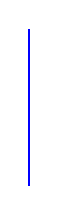
\begin{tikzpicture}[
gnuplot def/.append style={prefix={tikz/}}
]
\begin{scope}
\tikzset{
Nyquist grid/.style={black},
}
%\NyquistGraph[smooth,samples=81]{-2:4}
%{\IntAmp{\KB}}{\IntArg{\KB}}
\draw[color=blue,line width=0.3mm](0,0)--(0,-2);
\NyquistGrid
\end{scope}

\end{tikzpicture}
%\caption{$\textcolor{blue}{\zeta=\ZETA},\ \textcolor{red}{\zeta=\ZETAA}$}
\end{figure}

Esiste in realtà una singolarità nell'origine, si pensa di deformare l'asse
immaginario intorno l'origine con un arco di circonferenza di raggio
$\varepsilon$ ed angolo $\theta\in[0,\frac{\pi}{2}]$, dunque la precedente
equazione \ref{eq.polo_origine} diventa
$$
W(j\omega) = \frac{K_B}{\varepsilon e^{j\theta}}
$$
\begin{figure}[h]
\centering
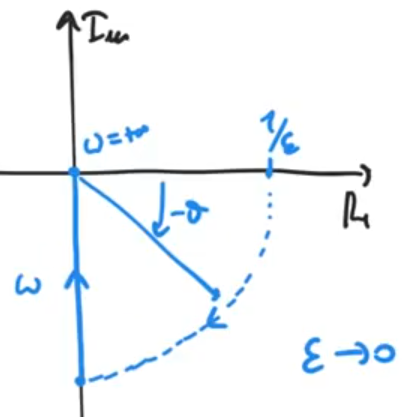
\includegraphics[width=\picwid]{approssimazione_epsilon_polo_origine}
\end{figure}

\newpage
\subsubsection{Esempio complesso}
Si ha la seguente funzione (in forma di Bode)
$$
W(s) = 10 \frac{1+0.1s}{(1+s)(1+10s)}
$$
Si ricavano i seguenti dati
$$
g=0,\ n-m=1,\ \tau_z=0.1,\ \tau_{p_1}=1,\
\tau_{p_2} = 10,\ K_B = 10
$$

\begin{figure}[h]
\centering
\begin{tikzpicture}[
gnuplot def/.append style={prefix={tikz/}},
xscale=7/3]
\begin{scope}[yscale=3/80]
\tikzset{
semilog lines/.style={black},
}
\OrdBode{10}
\UnitedB
\semilog{-2}{2}{-60}{20}
\BodeGraph[asymp
lines,samples=1000]{-2:2}{\POgAmpAsymp{1}{1}{0.1}{1}{9.999}+\POAmpAsymp{10}{1}}

\BodeGraph[samples=100]{-2:2}{\POgAmp{1}{1}{0.1}{1}{10}+\POAmp{10}{1}}

\end{scope}
\begin{scope}[yshift=-3.3cm,yscale=3/180]
\tikzset{
semilog lines/.style={black},
}
\UniteDegre
\OrdBode{15}
\semilog{-2}{2}{-180}{0}
\BodeGraph[samples=100]{-2:2}{\POgArg{1}{1}{0.1}{1}{10}+\POArg{10}{1}}

\BodeGraph[asymp lines,samples=1000]{-2:2}
{\POgArgAsymp{1}{1}{0.1}{1}{9.999}+\POArgAsymp{10}{1}}

\end{scope}
\end{tikzpicture}
%\caption{$\textcolor{red}{\tau=<0},\quad
%\textcolor{blue}{\tau=>0} $}
\end{figure}

Si rappresenta il conseguente diagramma di Nyquist.
\begin{figure}[h]
\centering
\begin{tikzpicture}[
gnuplot def/.append style={prefix={tikz/}},
scale=7/10
]
\begin{scope}
\tikzset{
Nyquist grid/.style={black},
}
\NyquistGraph[smooth,samples=100]{-3:2}
{\POgAmp{1}{1}{0.1}{1}{9.999}+\POAmp{10}{1}}
{\POgArg{1}{1}{0.1}{1}{9.999}+\POArg{10}{1}}

\NyquistPoint*[]{0.085/above,1/left,10/above left}
{\POgAmp{1}{1}{0.1}{1}{9.999}+\POAmp{10}{1}}
{\POgArg{1}{1}{0.1}{1}{9.999}+\POArg{10}{1}}

\NyquistGrid
\end{scope}

\end{tikzpicture}
%\caption{$\textcolor{blue}{\zeta=\ZETA},\ \textcolor{red}{\zeta=\ZETAA}$}
\end{figure}
Sono riportate sulla curva alcune frequenze per
notare come la distribuzione dei punti non sia uniforme.

\newpage
\subsubsection{Esempio poli del secondo ordine}
Si riporta un ulteriore esempio con un polo del secondo ordine al denominatore
$$
W(s) = 0.1\cdot\frac{1+10s}{1+0.6s+s^2}
$$

I valori caratteristici sono:
$$
K_B=0.1,\ \tau_z=10,\ \omega_n=1,\ \zeta=0.3<\frac{1}{\sqrt{2}},\ g=0,\ n-m=1
$$
\begin{figure}[h]
\centering
\begin{tikzpicture}[
gnuplot def/.append style={prefix={tikz/}},
xscale=7/3]
\begin{scope}[yscale=3/80]
\tikzset{
semilog lines/.style={black},
}
\OrdBode{10}
\UnitedB
\semilog{-2}{2}{-60}{20}
\BodeGraph[asymp
lines,samples=1000]{-2:2}{\SOAmpAsymp{0.1}{0.3}{1}-\POAmpAsymp{1}{9.999}}

\BodeGraph[samples=100]{-2:2}{\SOAmp{0.1}{0.3}{1}-\POAmp{1}{9.999}}

\end{scope}
\begin{scope}[yshift=-4.5cm,yscale=3/180]
\tikzset{
semilog lines/.style={black},
}
\UniteDegre
\OrdBode{15}
\semilog{-2}{2}{-90}{90}
\BodeGraph[samples=100]{-2:2}{\SOArg{0.1}{0.3}{1}-\POArg{1}{9.999}}

\BodeGraph[asymp lines,samples=1000]{-2:2}
{\SOArgAsymp{0.1}{0.3}{1}-\POArgAsymp{1}{9.999}}

\end{scope}
\end{tikzpicture}
%\caption{$\textcolor{red}{\tau=<0},\quad
%\textcolor{blue}{\tau=>0} $}
\end{figure}

Il basso valore di $\zeta$ causa la sovraelongazione della curva e il ripido
cambio di fase per $\omega=1$.

\newpage
Si rappresenta il diagramma di Nyquist
\begin{figure}[h]
\centering
\begin{tikzpicture}[
gnuplot def/.append style={prefix={tikz/}},
scale=25/10
]
\begin{scope}
\tikzset{
Nyquist grid/.style={black},
Nyquist label axis/.style={very thick,blue}
}
\NyquistGraph[smooth,samples=2000]{-3:2}
{\SOAmp{0.1}{0.3}{1}-\POAmp{1}{9.999}}
{\SOArg{0.1}{0.3}{1}-\POArg{1}{9.999}}


\NyquistPoint*[]{1/left,10/left}
{\SOAmp{0.1}{0.3}{1}-\POAmp{1}{9.999}}
{\SOArg{0.1}{0.3}{1}-\POArg{1}{9.999}}

\def\valgridNx{0.2}
\def\valgridNy{0.2}
\NyquistGrid

\end{scope}

\end{tikzpicture}
%\caption{$\textcolor{blue}{\zeta=\ZETA},\ \textcolor{red}{\zeta=\ZETAA}$}
\end{figure}

\subsubsection{Funzione con polo nell'origine}
Sia una funzione di trasferimento nella seguente forma con un solo polo
nell'origine
$$
W(s) = \frac{b_ms^m + \ldots + b_0}{s^n+a_{n-1}s^{n-1} + \ldots + a_1s}\qquad
\begin{aligned}
a_0 &= 0\\
g &= 1
\end{aligned}
$$

Il diagramma di Nyquist presenterà un asintoto
ortogonale all'asse reale passante per il punto $R_a$ calcolabile con la
seguente
$$
r_a = \frac{
\begin{vmatrix}
b_1 & b_0 \\
a_2 & a_1
\end{vmatrix}
}
{a_1^2}
$$

Si consideri la seguente funzione di trasferimento, si sviluppa il denominatore
$$
W(s) = \frac{K_B}{s(1+s)^2} = \frac{K_B}{s^3+2s^2 + s} =
\frac{b_0}{a_3s^3+a_2s^2 + a_1s}
$$
Si individuano i coefficienti della matrice
$$
r_a = \frac{
\begin{vmatrix}
0 & K_B\\
2 & 1
\end{vmatrix}
}
{1^2} = -2K_B
$$

\newpage
Si mostrano i diagrammi di Bode supponendo $K_B>0$
\begin{figure}[h]
\centering
\begin{tikzpicture}[
gnuplot def/.append style={prefix={tikz/}},
xscale=7/2]
\begin{scope}[yscale=3/80]
\tikzset{
semilog lines/.style={black},
}
\OrdBode{10}
\UnitedB
\semilog{-1}{1}{-60}{20}
\BodeGraph[asymp
lines,samples=1000]{-1:1}
{2*\POAmpAsymp{1}{1}+\IntAmp{1}}

\BodeGraph[samples=100]{-1:1}
{2*\POAmp{1}{1}+\IntAmp{1}}

\end{scope}
\begin{scope}[yshift=-1.5cm,yscale=3/180]
\tikzset{
semilog lines/.style={black},
}
\UniteDegre
\OrdBode{15}
\semilog{-1}{1}{-270}{-90}
\BodeGraph[samples=100]{-1:1}
{2*\POArg{1}{1}+\IntArg{1}}

\BodeGraph[asymp lines,samples=1000]{-1:1}
{2*\POArgAsymp{1}{1}+\IntArg{1}}

\end{scope}
\end{tikzpicture}
%\caption{$\textcolor{red}{\tau=<0},\quad
%\textcolor{blue}{\tau=>0} $}
\end{figure}

e quello di Nyquist
\begin{figure}[h]
\centering
\begin{tikzpicture}[
gnuplot def/.append style={prefix={tikz/}},
scale=15/10
]
\begin{scope}
\tikzset{
Nyquist grid/.style={black},
Nyquist label axis/.style={very thick,blue}
}
% \NyquistGraph[smooth,samples=100]{-3:0.8}
% {2*\POAmp{1}{1}+\IntAmp{1}}
% {2*\POArg{1}{1}+\IntArg{1}}

\NyquistGraph[smooth,samples=100]{-0.5:0.999}
{2*\POAmp{1}{1}+\IntAmp{1}}
{2*\POArg{1}{1}+\IntArg{1}}


% \NyquistPoint*[]{10/left}
% {2*\POAmp{1}{1}+\IntAmp{1}}
% {2*\POArg{1}{1}+\IntArg{1}}

\def\valgridNx{0.2}
\def\valgridNy{0.2}
\NyquistGrid

\end{scope}

\end{tikzpicture}
%\caption{$\textcolor{blue}{\zeta=\ZETA},\ \textcolor{red}{\zeta=\ZETAA}$}
\end{figure}

\newpage
\subsubsection{Funzione con ritardo}
Si aggiunge un ritardo $T$ ad una funzione di trasferimento con singolo polo
$$
W(s) = \frac{K_B}{1+s\tau}e^{-sT}
$$
non c'è alcun contributo al modulo che resta invariato
$$
|e^{j\omega T}| = 1 \forall \omega
$$
mentre la fase è traslata di $\omega T$
$$
\phase{e^{-j\omega T}} = -\omega T
$$

\def\T{10} %definizione ritardo T

\begin{figure}[h]
\centering
\begin{tikzpicture}[
gnuplot def/.append style={prefix={tikz/}},
xscale=7/2]
\begin{scope}[yscale=3/80]
\tikzset{
semilog lines/.style={black},
}
\OrdBode{10}
\UnitedB
\semilog{-1}{1}{-60}{20}
\BodeGraph[asymp
lines,samples=1000]{-1:1}
{\POAmpAsymp{1}{1}}

\BodeGraph[samples=100]{-1:1}
{\POAmp{1}{1}}

\end{scope}
\begin{scope}[yshift=-3cm,yscale=3/200]
\tikzset{
semilog lines/.style={black},
}
\UniteDegre
\OrdBode{20}
\semilog{-1}{1}{-200}{0}
\BodeGraph[samples=100]{-1:1}
{\POArg{1}{1}+\RetArg{\T}}

\BodeGraph[asymp lines,samples=1000]{-1:1}
{\POArgAsymp{1}{1}+\RetArg{\T}}

\end{scope}
\end{tikzpicture}
\caption{$T = \T $}
\end{figure}

Si osserva come il diagramma del modulo resti invariato mentre quello della
fase decresce all'aumentare di $\omega$.

\newpage
Questa differenza può essere apprezzata nel diagramma di Nyquist

\begin{figure}[h]
\centering
\begin{tikzpicture}[
gnuplot def/.append style={prefix={tikz/}},
scale=20/10
]
\begin{scope}
\tikzset{
Nyquist grid/.style={black},
Nyquist label axis/.style={very thick,blue}
}
% \NyquistGraph[smooth,samples=100]{-3:0.8}
% {2*\POAmp{1}{1}+\IntAmp{1}}
% {2*\POArg{1}{1}+\IntArg{1}}

\NyquistGraph[smooth,samples=100]{-2:2}
{\POAmp{1}{1}}
{\POArg{1}{1}+\RetArg{\T}}


% \NyquistPoint*[]{10/left}
% {2*\POAmp{1}{1}+\IntAmp{1}}
% {2*\POArg{1}{1}+\IntArg{1}}

\def\valgridNx{0.2}
\def\valgridNy{0.2}
\NyquistGrid

\end{scope}

\end{tikzpicture}
\caption{$T=\T,\ K_B=1$}
\end{figure}

In questo caso il ritardo è contenuto e il sistema converge comunque
nell'origine nonostante la porzione di grafico presente nel secondo quadrante,
potrebbe accadere invece che la curva passi all'esterno del punto $(-1,0)$ e il
sistema risulti instabile, esiste dunque un limite al guadagno $K_B$ che si può
imporre ad un sistema con ritardo.
\begin{figure}[h]
\centering
\def\T{20}
\begin{tikzpicture}[
gnuplot def/.append style={prefix={tikz/}},
scale=20/10
]
\begin{scope}
\tikzset{
Nyquist grid/.style={black},
Nyquist label axis/.style={very thick,blue}
}
% \NyquistGraph[smooth,samples=100]{-3:0.8}
% {2*\POAmp{1}{1}+\IntAmp{1}}
% {2*\POArg{1}{1}+\IntArg{1}}

\NyquistGraph[smooth,samples=1000]{-2:2}
{\POAmp{2}{1}}
{\POArg{2}{1}+\RetArg{\T}}


% \NyquistPoint*[]{10/left}
% {2*\POAmp{1}{1}+\IntAmp{1}}
% {2*\POArg{1}{1}+\IntArg{1}}

\def\valgridNx{0.2}
\def\valgridNy{0.2}
\NyquistGrid

\end{scope}

\end{tikzpicture}
\caption{$T=\T,\ K_B=2$}
\end{figure}
